% =============================================================================
% A Computational Readability Evaluation for Assessing AI Transcription
% Readiness of Physical Documents
%
% IEEE conference format (IEEEtran), numbered IEEE-style citations.
% Overleaf: upload main.tex, references.bib, and the figures/ folder.
% Compiler: pdfLaTeX. Bibliography: BibTeX with IEEEtran.bst (built into
% Overleaf). If you prefer a hand-written reference list, delete the two
% \bibliography lines at the end and paste in references_ieee.tex instead.
%
% Red [bracketed] text marks facts only the authors can supply. Search for
% \todo to find them all before submitting.
% =============================================================================
\documentclass[conference]{IEEEtran}

\usepackage{cite}
\usepackage{amsmath}
\usepackage{graphicx}
\usepackage{booktabs}
\usepackage[table]{xcolor}
\usepackage[caption=false,font=footnotesize]{subfig}
\usepackage{url}

\graphicspath{{figures/}}

\newcommand{\todo}[1]{\textcolor{red}{[#1]}}

\begin{document}

\title{A Computational Readability Evaluation for Assessing AI Transcription
Readiness of Physical Documents}

\author{\IEEEauthorblockN{\todo{Authors}}
\IEEEauthorblockA{\todo{Affiliations and emails}}}

\maketitle

% =============================================================================
\begin{abstract}
The accuracy of optical character recognition (OCR) output depends in part on
the quality and legibility of the original physical document. Preprocessing
improves the quality of scanned images, but it is computationally expensive to
run on every scan in a large collection. Evaluating each document's readability
in advance shows which ones need additional processing before transcription.
This paper presents an approach for assessing the machine readability of
handwritten scientific documents, with a preliminary implementation and
evaluation of a quantitative readability score. The approach uses three
computational metrics to score the baseline consistency, spatial organization,
and text fragmentation of one page from each of three handwritten chemistry lab
notebooks kept by students studying metal organic frameworks (MOFs). These
notebooks are categorized as having neat, average, and messy handwriting and
are scored on a scale from 0 (low readability) to 1 (high readability). The
resulting score is then compared to transcription accuracy, measured as the
character error rate (CER) of an OCR transcription against a ground truth typed
by the authors. The readability score ranked the pages in the same order as the
CER (Pearson $r = -0.882$; Spearman $\rho = -1.000$): pages with a higher
readability score had lower transcription error. OCR confidence, the OCR
tool's own estimate of how reliable its output is, was by contrast positively
correlated with CER ($r = 0.674$; $\rho = 0.500$). However, all scores fell
within a narrow range and error rates were high for every page (68--77\% CER),
so this study should serve as a first test of the approach. This methodology
should help prioritize preprocessing and inform evidence-based recommendations
for documentation practices that support the machine readability of handwritten
scientific documents.
\end{abstract}

% =============================================================================
\section{Introduction}

Handwritten lab notebooks are both records of experiments and documentation of
student learning. For this information to be used by researchers and in AI
analysis, it must first be digitized. Converting these lab notebooks or other
handwritten documents into digital transcriptions depends on the application of
optical character recognition (OCR) tools to scanned copies of the lab
notebooks' pages. The accuracy of these tools, however, depends partly on the
quality of the input provided \cite{ye2013, alaei2024}. Preprocessing
scans of handwritten documents can improve input quality and make a document
more machine-readable \cite{sauvola2000, gonzalez2018}, but is
an expensive process in computing time and effort for large collections
\todo{citation needed, or rephrase as the authors' observation}. Because there
is no simple way to determine which scans may require preprocessing, assessing
each notebook's readability before transcription would enhance the
transcription pipeline's efficiency.

The notebooks used in this study originate from the Reticular Synthesis and
Materials Design Lab (RSMDL) of Dr.\ Fernando Uribe-Romo of the University of
Central Florida's Chemistry Department, which studies metal organic frameworks
(MOFs). The effort to digitize these notebooks is a part of the NSF-HDR
Institute for Data-Driven Dynamical Design in conjunction with the Metadata
Research Center at Drexel University. Earlier work using MOF students' lab
notebooks returned table-cell error rates of 4\% to 18\%, depending on the OCR
tool used for transcription and the correction steps taken
\cite{pepper2025}, and these results support checking scan quality
before transcription.

This paper presents a preliminary approach to assessing handwritten scientific
documents for machine readability before OCR transcription. The section that
follows provides a brief background on the use of analog notebooks in labs,
defines Computational Archival Science (CAS), and details how it relates to our
research. Next, we state our research goals and describe the methods used to
compute a readability score from three measurements (baseline consistency,
spatial organization, and text fragmentation). As part of our approach, the
score is then compared to the character error rate (CER) of an OCR
transcription, to check whether the score tracks actual transcription error.
Finally, we discuss research implications and future work, identify next
steps, and present our conclusions.

% =============================================================================
\section{Background: Analog Lab Notebooks and CAS}

Low barrier to adoption and use, reasonable cost, and portability are the
principal reasons why scientists use physical lab notebooks in wet labs instead
of electronic ones \cite{kanza2017}. In addition to these advantages,
handwritten historical documents and modern physical records do not depend on
software and can outlast rapidly evolving technology \cite{ryan2007}.
However, to be shared, reproduced, and analyzed, physical lab notebooks and
other handwritten documents must be digitally transcribed. Transcription at
scale requires a reliable transcription pipeline so that the data remain
accurate and the processing time reasonable.
% Comment [6] is still assigned to David for this sentence.

Computational Archival Science (CAS) addresses the need for the efficient and
reliable processing of records by combining archival science, computer science,
and subject expertise to develop scalable and automated methods for management
\cite{marciano2018}. A lab notebook can be defined as an archival
record since it documents the steps, observations, and results of an
experiment. This observation draws from foundational archival theory, which
holds that a record's meaning depends on its provenance (the context in which
it was created) and its original order (the sequence in which it was kept)
\cite{jenkinson1922}. CAS principles call for archival records such as
these to remain reliable and authentic, as well as connected to their original
context, when converted to digital form \cite{hedges2022}. Our proposed
readability score aims to support reliability by identifying which scans
require further processing. This allows the visual quality of the scans to be
improved before transcription, which makes the output more accurate and keeps
the transcription pipeline efficient.

% =============================================================================
\section{Goals and Objectives}

An overall motivating goal of our research is to create a method by which
physical lab notebooks may be reliably transcribed and ultimately added to a
database that can be queried with pedagogical inquiries and mined for
additional information and insights. The immediate goal of the research
presented in this paper is to define an approach for assessing the machine
readability of scanned handwritten lab notebooks using computational methods
before OCR transcription. The goal has three objectives:
\begin{itemize}
  \item Measure baseline consistency, spatial organization, and text
        fragmentation from scanned notebook pages without using an OCR tool.
  \item Combine the resulting measurements into a single readability score on a
        scale of 0 (low readability) to 1 (high readability).
  \item Compare the readability score to the CER of OCR transcriptions from
        notebooks categorized as neat, average, and messy handwriting.
\end{itemize}

% =============================================================================
\section{Methods}
\label{sec:methods}

To address our goals, this study developed and evaluated a computational method
for quantifying structural characteristics, to determine whether the measurable
visual properties of laboratory notebook pages can predict OCR transcription
performance without using the OCR tool itself. The methodology was informed by
research on the variability of handwriting
\cite{papavassiliou2010, rabaev2026}, prior work on
scientific document recognition \cite{pepper2025}, document image
quality \cite{ye2013, alaei2024}, and OCR evaluation
\cite{smith2007, levenshtein1966}. These areas guided the
selection of structural features and validation metrics.

\subsection{Data}
\label{sec:data}

This preliminary study uses three pages: one representative page
($1455 \times 1980$ pixels) from each of three student lab notebooks. A MOF
researcher visually assessed the notebook scans and grouped them by handwriting
style as neat, average, or messy (Fig.~\ref{fig:styles}).

\begin{figure*}[t]
  \centering
  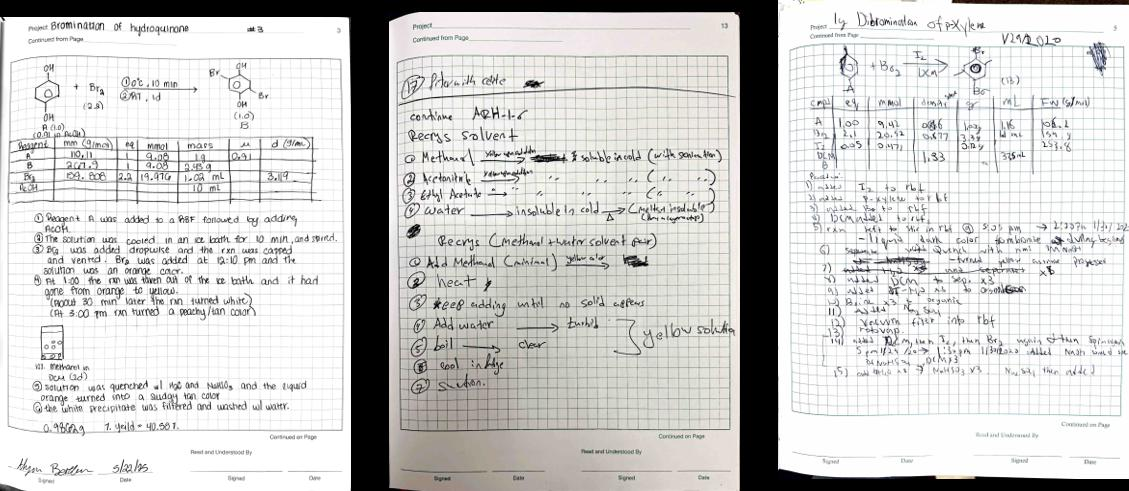
\includegraphics[width=0.85\textwidth]{fig1_handwriting_styles.png}
  \caption{Neat, average, and messy handwriting styles (left to right) from
  students' chemistry lab notebooks from Dr.\ Fernando Uribe-Romo's lab at the
  University of Central Florida.}
  \label{fig:styles}
\end{figure*}

Each page was prepared (Section~\ref{sec:methods}-\ref{sec:prep}) using
grayscale conversion, adaptive thresholding, and morphological opening. Three
structural measurements were taken from the prepared image: baseline
consistency ($b$), spatial organization ($s$), and text fragmentation ($f$).
These were combined into a readability score using a weighted formula,
resulting in a value from 0 (low readability) to 1 (high readability). All
image processing used Python 3.13 and OpenCV \cite{bradski2000}.

To test whether higher readability scores coincide with lower transcription
error, each original, unprepared scan was transcribed with Tesseract OCR
\todo{version} \cite{smith2007, tesseract_manual} through the
pytesseract library \cite{pytesseract}, using default settings (English
model, automatic page segmentation). The ground truth for each page is a
manual transcription typed by the authors, who entered the text of each scan
into a plain UTF-8 text file, keeping the page's line breaks and reading order;
no OCR output was used to create it. CER was computed with the JiWER library
\cite{jiwer} as the number of character substitutions, deletions, and
insertions \cite{levenshtein1966} needed to turn the OCR output into the
ground truth, divided by the number of ground-truth characters (997, 463, and
845 for the neat, average, and messy pages). Case and punctuation were kept,
and no other text normalization was applied.
% Optional disclosure: "Line breaks in the ground truth were compared against
% the single spaces that join OCR words, which raises CER slightly; collapsing
% all whitespace lowers CER by 0.2 to 2.8 points and does not change the page
% ranking."

OCR confidence is the mean of the word-level confidence scores (0 to 100) that
Tesseract reports through \texttt{pytesseract.image\_to\_data}, averaged over
all words on the page and excluding the $-1$ values Tesseract assigns to
non-word layout entries. OCR confidence was compared with both the readability
score and the CER.

\subsection{Image Preparation}
\label{sec:prep}

OCR transcription accuracy depends, in part, on how effectively the system can
distinguish between handwritten text and the surrounding document image.
Inconsistencies such as background shadows, uneven illumination of the scanned
page, page texture, and isolated image noise can be mistaken for handwriting
and hinder the detection of actual handwritten characters
\cite{smith2007}. For example, a faint decimal point can be lost
during thresholding, while disconnected strokes can cause a single character to
be represented as several separate components in the image
\cite{fujisawa1992}. Similarly, adjacent characters can merge into
one foreground region, making segmentation more difficult. Errors such as these
can propagate through the OCR transcription pipeline and raise the error rate
of the final transcription. Following Alaei \emph{et al.} \cite{alaei2024}, we treat document
image quality as affecting both structural feature extraction and OCR
performance. Image preparation removes this noise so that it does not distort
the final readability score.

\begin{figure}[t]
  \centering
  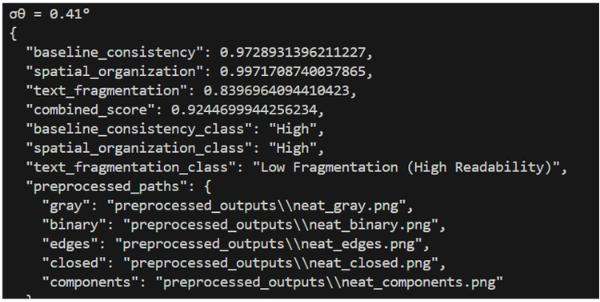
\includegraphics[width=\columnwidth]{fig2_script_output.png}
  \caption{Readability scoring output (Python 3.13) for the neat notebook page:
  baseline angle deviation ($\sigma_\theta$), the three metric scores, the
  combined score, and the class of each metric from Table~\ref{tab:bands}.}
  \label{fig:output}
\end{figure}

The first preparation stage, grayscale conversion, reduces each pixel from
three color channels to a single intensity value, which simplifies the analysis
when ink color is not being evaluated \cite{gonzalez2018}. Before
thresholding, a $3 \times 3$ Gaussian blur smooths small pixel-level variations
\cite{gonzalez2018, opencv_filtering}. Adaptive thresholding then separates
the handwriting from the background by computing a separate threshold for each
pixel from a Gaussian-weighted $31 \times 31$ pixel neighborhood with an offset
of 11 gray levels \cite{opencv_misc}: a pixel is treated as ink if
it is at least 11 levels darker than the weighted average of the area around
it. These two settings were chosen by visual inspection of the thresholded
output, and they affect the resulting scores (Section~\ref{sec:discussion}).
% Confirm with Simm that 31 and 11 were tuned by eye.
Unlike global thresholding, which applies one threshold across the entire
image, adaptive thresholding responds to local variations in illumination,
which is particularly useful for scanned documents
\cite{sauvola2000, bradley2007, binmakhashen2019}.
The threshold is inverted, so ink becomes white (foreground) and paper becomes
black (background), because OpenCV's morphology and connected-component
functions treat nonzero (white) pixels as the object being measured
\cite{opencv_morph, opencv_shape}.

Morphological processing provides an additional means of controlling the shape
and connectivity of foreground regions
\cite{serra1982, haralick1987}. Morphological opening,
erosion followed by dilation, removes isolated foreground specks smaller than
its kernel ($3 \times 3$, one pass), which reduces the likelihood that image
noise will be interpreted as handwriting later in the analysis
\cite{haralick1987, gonzalez2018}. Conversely, morphological
closing, dilation followed by erosion, reconnects nearby foreground strokes
\cite{haralick1987, gonzalez2018}. Closing ($5 \times 5$ kernel,
two passes) is applied only when measuring text fragmentation
(Section~\ref{sec:methods}-\ref{sec:measure}).

\begin{figure*}[t]
  \centering
  \subfloat[]{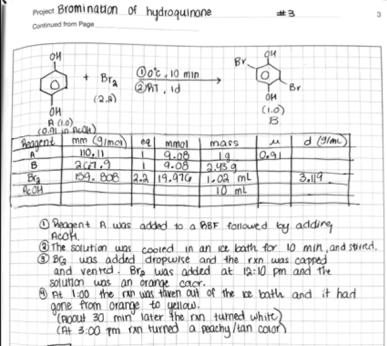
\includegraphics[width=0.19\textwidth]{fig3a_grayscale.png}}\hfill
  \subfloat[]{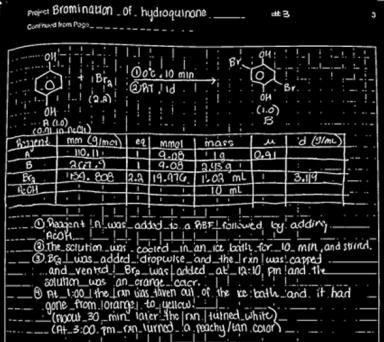
\includegraphics[width=0.19\textwidth]{fig3b_threshold_opening.png}}\hfill
  \subfloat[]{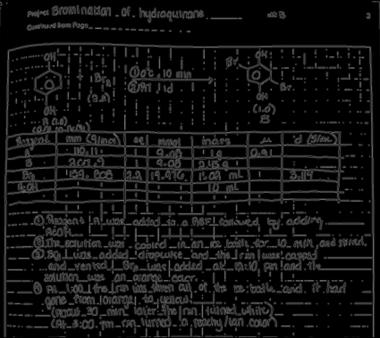
\includegraphics[width=0.19\textwidth]{fig3c_canny_edges.png}}\hfill
  \subfloat[]{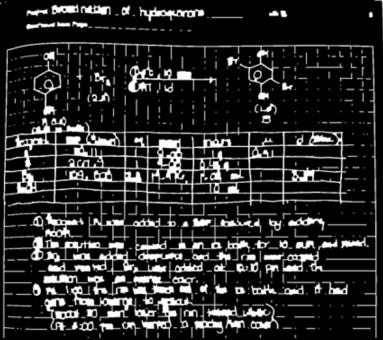
\includegraphics[width=0.19\textwidth]{fig3d_closing.png}}\hfill
  \subfloat[]{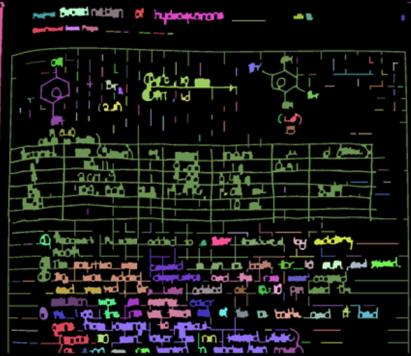
\includegraphics[width=0.19\textwidth]{fig3e_components.png}}
  \caption{Image preparation for the neat notebook page, in processing order.
  (a) Grayscale conversion of the original scan.
  (b) Adaptive thresholding (inverted) followed by morphological opening; ink is
  white because OpenCV measures nonzero pixels as foreground.
  (c) Canny edge map of (b) \cite{canny1986}, shown for illustration only;
  no metric uses it.
  (d) Morphological closing of (b), which joins nearby strokes before text
  fragmentation is measured.
  (e) Connected components of (d), each shown in a different color.}
  \label{fig:prep}
\end{figure*}

\subsection{Readability Measurements}
\label{sec:measure}

Handwritten documents inherently vary in baseline position, inter-line spacing,
character size, and character overlap, which complicate text-line segmentation
and recognition \cite{papavassiliou2010, rabaev2026}.
Following image preparation, three structural metrics are computed: baseline
consistency ($b$), spatial organization ($s$), and text fragmentation ($f$).

Each raw measurement is converted to a 0 to 1 score by comparing it with a
fixed \emph{reference value}, the point at which the score reaches 0 (or, for
the fragmentation terms, the point at which a term reaches its maximum).
Results outside 0 to 1 are clipped, and higher scores always mean higher
readability. The reference values were chosen by the authors' judgement rather
than derived from data or prior work, and are listed in
Table~\ref{tab:reference}.

\begin{itemize}
  \item \textbf{Baseline consistency ($b$).} A horizontal projection profile
  (the count of ink pixels in each row) locates the bands of text on the page
  \cite{likforman2007, papavassiliou2010}. Connected
  components of at least 15 pixels are assigned to the band containing their
  center, and bands with fewer than four components are skipped. For each
  band, a least-squares line is fitted through the bottom-center points of its
  components \cite{ogorman1993, opencv_shape}; fits whose points lie
  more than 8 pixels from the line on average are rejected. The baseline angle
  deviation $\sigma_\theta$ is the standard deviation of the fitted line
  angles, weighted by the number of components in each line, and
  \[ b = 1 - \frac{\sigma_\theta}{15^\circ}. \]
  A page whose lines all share one angle scores 1; a page whose line angles
  vary by $15^\circ$ or more scores 0.

  \item \textbf{Spatial organization ($s$).} Rows whose ink count exceeds 15\%
  of the page's fullest row are grouped into bands, and the vertical distance
  between the centers of consecutive bands is measured
  \cite{likforman2007}. With $\mathrm{Var}(d)$ the variance of these
  spacings and $H$ the page height in pixels,
  \[ s = 1 - \frac{\mathrm{Var}(d)}{H^2/16}. \]
  The reference $H^2/16$ corresponds to a spacing standard deviation of one
  quarter of the page height (495 pixels for these pages). Low spacing variance
  means better organization and fewer OCR segmentation errors.

  \item \textbf{Text fragmentation ($f$).} After morphological closing,
  connected components smaller than 15 pixels are discarded as noise. Three
  terms are computed, each oriented so that a larger value means more
  fragmentation, and each limited to 0 to 1:
  \begin{itemize}
    \item component density $D = \min(40\,n/A,\ 1)$, where $n$ is the number
    of components and $A$ is their total ink area in pixels
    \cite{fujisawa1992};
    \item nearest-neighbor dispersion $N = \min(\bar{r}/\sqrt{HW},\ 1)$, where
    $\bar{r}$ is the mean distance from each component's centroid to its
    nearest neighbor and $\sqrt{HW}$ is the square root of the page area; larger
    distances suggest more scattered text
    \cite{ogorman1993, clark1954};
    \item small-component ratio $R$, the share of components under 150 pixels,
    such as broken strokes, isolated punctuation, and residual noise
    \cite{fujisawa1992, ye2013}.
  \end{itemize}
  The terms are combined into a fragmentation index, which is subtracted from 1
  so that higher $f$ means less fragmentation and higher readability:
  \[ f = 1 - \left(0.45\,D + 0.35\,N + 0.20\,R\right). \]
  These weights were chosen by judgement, as no published source or empirical
  data in this study's corpus established the relative contributions of the
  three terms. The resulting score is therefore exploratory and should not be
  interpreted as a fully validated measure of readability.
\end{itemize}

\begin{table*}[t]
  \centering
  \caption{Reference values used to scale each raw measurement to 0--1. All
  were chosen by the authors' judgement.}
  \label{tab:reference}
  \small
  \begin{tabular}{@{}lll@{}}
    \toprule
    Metric or term & Raw measurement & Reference value \\
    \midrule
    $b$       & SD of line angles, $\sigma_\theta$ & $15^\circ$ ($b = 0$ at or above) \\
    $s$       & Variance of band spacing           & $H^2/16$ (SD of 495 px) \\
    $f$: $D$  & Components per ink pixel           & $\times 40$, capped at 1 \\
    $f$: $N$  & Mean nearest-neighbor distance     & $\sqrt{HW}$ (1697 px) \\
    $f$: $R$  & Share of components $< 150$ px     & None (already a proportion) \\
    \bottomrule
  \end{tabular}
\end{table*}

\subsection{Combined Readability Score}
\label{sec:combined}

The three metrics are combined as
\[ \text{Score} = 0.40\,b + 0.20\,s + 0.40\,f. \]
Because the weights sum to 1 and each metric lies between 0 and 1, the combined
score also lies between 0 and 1. The weights reflect the authors' judgement
that line alignment and stroke fragmentation affect OCR more directly than the
spacing between lines; no prior work supplies weights for these metrics. Each
metric and the combined score are labelled High, Moderate, or Low using the
bands in Table~\ref{tab:bands}. The cut-offs at 0.80 and 0.50 were also chosen
by the authors' judgement.

\begin{table}[t]
  \centering
  \caption{Classification bands applied to each metric and to the combined
  score.}
  \label{tab:bands}
  \small
  \begin{tabular}{@{}lll@{}}
    \toprule
    Score & $b$, $s$, and combined & $f$ \\
    \midrule
    \rowcolor{green!15}
    0.80--1.00 & High     & Low fragmentation \\
    \rowcolor{yellow!20}
    0.50--0.79 & Moderate & Moderate fragmentation \\
    \rowcolor{red!12}
    0.00--0.49 & Low      & High fragmentation \\
    \bottomrule
  \end{tabular}
\end{table}

Finally, the readability score was compared with the CER and with OCR
confidence using Pearson's $r$ and Spearman's $\rho$.

% =============================================================================
\section{Results}
\label{sec:results}

Results are based on one page from each of three student lab notebooks
(Table~\ref{tab:raw}). Combined readability scores all fell within the High
readability band, between 0.920 and 0.924. The pages ranked in the same order
by combined score as by CER (neat, average, messy), giving a negative
relationship between the readability score and CER (Pearson $r = -0.882$;
Spearman $\rho = -1.000$; Table~\ref{tab:corr}). OCR confidence had a positive
correlation with CER ($r = 0.674$; $\rho = 0.500$), and the correlation between
the readability score and OCR confidence was $r = -0.247$, $\rho = -0.500$.

\begin{table*}[t]
  \centering
  \caption{Readability metrics, CER, and OCR confidence for each page.}
  \label{tab:raw}
  \small
  \begin{tabular}{@{}lcccccc@{}}
    \toprule
    Page & $b$ & $s$ & $f$ & Combined & CER & OCR confidence \\
    \midrule
    Neat    & 0.9729 & 0.9972 & 0.8397 & 0.9245 & 67.7\% & 54.6 \\
    Average & 0.9728 & 0.9975 & 0.8350 & 0.9226 & 75.6\% & 79.9 \\
    Messy   & 0.9406 & 0.9977 & 0.8599 & 0.9197 & 77.2\% & 63.9 \\
    \bottomrule
  \end{tabular}
\end{table*}

\begin{table}[t]
  \centering
  \caption{Correlations between readability score, OCR confidence, and CER
  ($n = 3$).}
  \label{tab:corr}
  \small
  \begin{tabular}{@{}lcc@{}}
    \toprule
    Comparison & Pearson $r$ & Spearman $\rho$ \\
    \midrule
    Combined score vs.\ OCR confidence & $-0.247$ & $-0.500$ \\
    Combined score vs.\ CER            & $-0.882$ & $-1.000$ \\
    OCR confidence vs.\ CER            & $0.674$  & $0.500$  \\
    \bottomrule
  \end{tabular}
\end{table}

Baseline consistency remained high for all pages but had the widest spread of
the three metrics (0.941 to 0.973), and it was the only metric that placed the
messy page last. With three pages, none of the correlations is statistically
significant (combined score vs.\ CER: Pearson $p = 0.31$; Spearman exact
two-sided $p = 0.33$). With $n = 3$, the smallest attainable Spearman $p$-value
is 0.33, so these correlations describe the ranking of these three pages only.

% =============================================================================
\section{Discussion}
\label{sec:discussion}

With this research, we have started to address our goal of assessing the
machine readability of handwritten lab notebooks before transcription. The
readability score, derived from computational methods independent of the OCR
tool, ranked the scanned pages in the same order as the CER and the visual
assessment (Table~\ref{tab:raw}): pages with higher structural readability
scores had lower OCR transcription error.

While the readability score ranked the pages in the same order as the CER,
every page was rated High readability despite CERs of 68\% to 77\%. This was
our biggest surprise, as identifying scanned images that may be unreadable to
machines is our main use case. Spatial organization ($s$) varied by less than
0.001 across the three pages (0.997 to 0.998). Its reference value, a spacing
standard deviation of 495 pixels, is about twenty times larger than the
spacing variation measured (24 to 26 pixels), so nearly any page scores close
to 1. All three notebooks are also written on printed grid paper, and the
projection profile appears to detect the grid rows along with the handwriting
(on the average page it found 64 bands about 30 pixels apart), which makes line
spacing look similar on every page. Scaling spacing against each page's own
mean line spacing, and removing printed grid lines before measurement, should
make $s$ more informative.

Text fragmentation ($f$) rated the notebook categorized as messy as the least
fragmented, which contradicts the visual nature of messy handwriting. This is
not caused by the direction of the formula, since each term increases with
fragmentation and the weighted sum is subtracted from 1. On the average page,
the small-component ratio supplied 88\% of the fragmentation index (0.145 of
0.165), while component density (0.008) and nearest-neighbor dispersion
(0.012) contributed little, because their reference values are much larger
than the values measured. The small components appear to be dominated by
fragments of the printed grid, which thresholding and opening break into short
dashes (Fig.~\ref{fig:prep}b). The messy notebook's darker grid and hand-drawn
table survive thresholding as long connected lines, which would produce fewer
small components and therefore a higher $f$.
\todo{Confirm with src/metric\_components.py on the neat and messy pages and
replace ``appear to'' and ``would'' with the measured values.}
We also found that baseline consistency ($b$) was the factor most aligned with
the visual assessment for this set, with the messy notebook ranking lowest.

OCR confidence did not track CER on these pages. The neat page had the lowest
confidence (54.6) but the lowest error (67.7\%), and the average page had the
highest confidence (79.9) but the second-highest error (75.6\%). With three
pages this is an observation rather than a finding, but it suggests that OCR
confidence alone may not reflect transcription accuracy and should be used with
care as a signal of document readability.

This study has four limitations: small sample size, judgement-based weights
and settings, uncalibrated reference values, and the use of one OCR tool.
First, we tested the method on three pages, one from each notebook; because a
sample this size cannot establish significant results, this study should be
seen as an early test of the approach. Second, the weights and preparation
settings were chosen by judgement, and the results are sensitive to them. With
the weight on $s$ held at 0.20, the page ranking matches the CER ranking only
when the weight on $b$ is between 0.35 and 0.80, and $f$ on its own ranks the
messy page as most readable. Changing the thresholding neighborhood and offset
moved the average page's combined score between 0.885 and 0.933 across the
settings we tested, a wider range than the difference between pages. Third,
the reference values compress all pages into a narrow band near the top of the
scale; calibrating them on a larger set of pages (for example, setting each
reference at a high percentile of the observed values) is needed before the
High, Moderate, and Low labels are meaningful. Lastly, the transcription
software Tesseract produced high error rates on every page, including the page
judged neat both visually and by the combined score, which suggests that future
work should compare multiple transcription tools.

% =============================================================================
\section{Conclusion}

In this paper, we propose an approach for assessing the machine readability of
scanned handwritten lab notebooks prior to OCR transcription. This approach
uses image processing to quantify baseline consistency, spatial organization,
and text fragmentation. The results are then combined into a score that
reports on the document's machine readability without the use of OCR, which
can be expensive or time-consuming to run at scale. In a preliminary test on
three scanned notebook pages, the score ranked the pages in the same order as
their CER, while OCR confidence did not track transcription accuracy.

The next steps in this research are to (1) test a wider range of pages,
including pages expected to score low; (2) calibrate the reference values and
weights on that larger set rather than by judgement; (3) revise text
fragmentation by removing printed grid and ruling lines before measurement and
rescaling its density and nearest-neighbor terms, which currently contribute
little; and (4) compare several OCR tools.

This work makes progress toward quantifying notebook and handwriting quality, a
step that our earlier work identified as necessary for making analog lab
notebooks more AI-ready \cite{pepper2025}. With a readability check that
could reliably predict transcription accuracy before OCR, notebooks that have
never been transcribed could be selected for transcription pipelines or
identified for further preprocessing. Digital transcription enables physical
documents to be added to searchable databases where they may be studied and
used by scientists, teachers, and students alike. In time, these
transcriptions may aid in training future tools and inform future physical
documentation practices.

% =============================================================================
\section*{Acknowledgment}

This work was supported by the National Science Foundation through the
Institute for Data-Driven Dynamical Design, OAC-2118201, and the Drexel
University Metadata Research Center. We acknowledge the original authors of the
lab notebooks, Alyssa Bordner, Yuen Lau, and Wesley Newsome, and the
Uribe-Romo lab.

\bibliographystyle{IEEEtran}
\bibliography{references}

\end{document}
